% Generated by LitigCharts.PublicationFigures. Captions and provenance are sidecars.
\documentclass[10pt,tikz,border=5pt]{standalone}
\usepackage{lmodern}
\usetikzlibrary{patterns}
\begin{document}
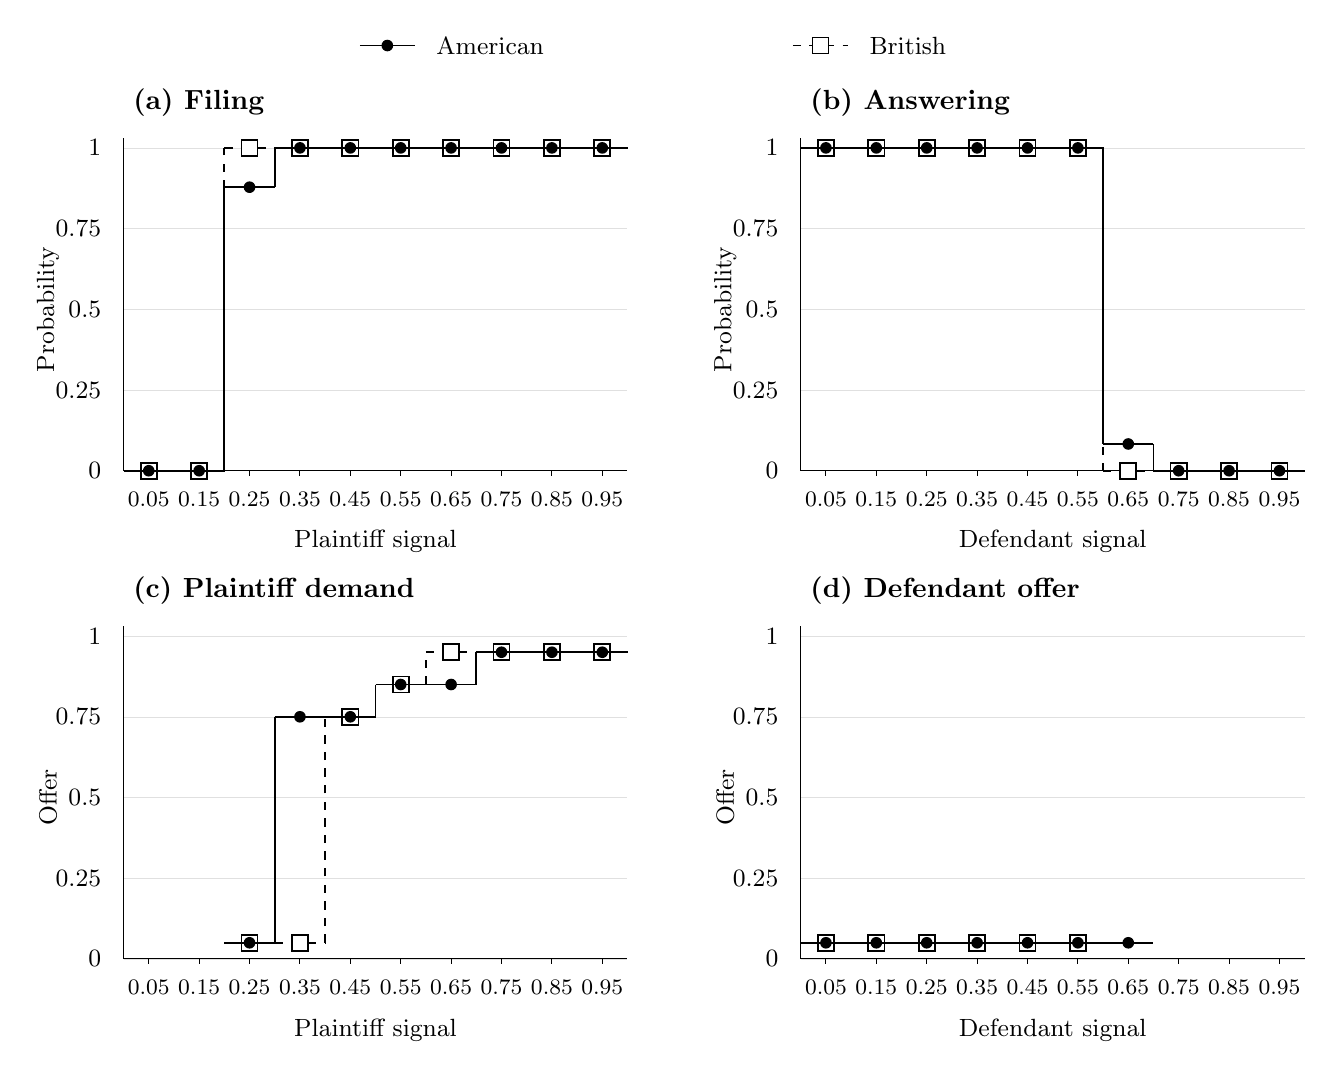
\begin{tikzpicture}[font=\small]\draw[black,solid,line width=.65pt] (4,12) -- (4.7,12);
\fill[black] (4.35,12) circle[radius=2.1pt];
\node[anchor=west] at (4.85,12) {American};
\draw[black,dashed,line width=.65pt] (9.5,12) -- (10.2,12);
\node[draw=black,fill=white,rectangle,inner sep=0pt,minimum size=5.8pt,line width=.6pt] at (9.85,12) {};
\node[anchor=west] at (10.35,12) {British};
\begin{scope}[shift={(1,6.6)},x=6.4cm,y=4.1cm]
\node[anchor=west,font=\bfseries] at (0,1.14) {(a) Filing};
\draw[black!12,line width=.2pt] (0,0) -- (1,0);
\node[anchor=east] at (-.025,0) {0};
\draw[black!12,line width=.2pt] (0,0.25) -- (1,0.25);
\node[anchor=east] at (-.025,0.25) {0.25};
\draw[black!12,line width=.2pt] (0,0.5) -- (1,0.5);
\node[anchor=east] at (-.025,0.5) {0.5};
\draw[black!12,line width=.2pt] (0,0.75) -- (1,0.75);
\node[anchor=east] at (-.025,0.75) {0.75};
\draw[black!12,line width=.2pt] (0,1) -- (1,1);
\node[anchor=east] at (-.025,1) {1};
\draw[black,line width=.4pt] (0,1.03) -- (0,0) -- (1,0);
\draw ( 0.05,0) -- (0.05,-.016);
\node[anchor=north,font=\footnotesize] at (0.05,-.035) {0.05};
\draw ( 0.15,0) -- (0.15,-.016);
\node[anchor=north,font=\footnotesize] at (0.15,-.035) {0.15};
\draw ( 0.25,0) -- (0.25,-.016);
\node[anchor=north,font=\footnotesize] at (0.25,-.035) {0.25};
\draw ( 0.35,0) -- (0.35,-.016);
\node[anchor=north,font=\footnotesize] at (0.35,-.035) {0.35};
\draw ( 0.45,0) -- (0.45,-.016);
\node[anchor=north,font=\footnotesize] at (0.45,-.035) {0.45};
\draw ( 0.55,0) -- (0.55,-.016);
\node[anchor=north,font=\footnotesize] at (0.55,-.035) {0.55};
\draw ( 0.65,0) -- (0.65,-.016);
\node[anchor=north,font=\footnotesize] at (0.65,-.035) {0.65};
\draw ( 0.75,0) -- (0.75,-.016);
\node[anchor=north,font=\footnotesize] at (0.75,-.035) {0.75};
\draw ( 0.85,0) -- (0.85,-.016);
\node[anchor=north,font=\footnotesize] at (0.85,-.035) {0.85};
\draw ( 0.95,0) -- (0.95,-.016);
\node[anchor=north,font=\footnotesize] at (0.95,-.035) {0.95};
\node[rotate=90] at (-.15,.5) {Probability};
\node at (.5,-.22) {Plaintiff signal};
\draw[black,dashed,line width=.65pt] (0,0) -- (0.1,0);
\node[draw=black,fill=white,rectangle,inner sep=0pt,minimum size=5.8pt,line width=.6pt] at (0.05,0) {};
\draw[black,dashed,line width=.65pt] (0.1,0) -- (0.2,0);
\draw[black,dashed,line width=.65pt] (0.1,0) -- (0.1,0);
\node[draw=black,fill=white,rectangle,inner sep=0pt,minimum size=5.8pt,line width=.6pt] at (0.15,0) {};
\draw[black,dashed,line width=.65pt] (0.2,1) -- (0.3,1);
\draw[black,dashed,line width=.65pt] (0.2,0) -- (0.2,1);
\node[draw=black,fill=white,rectangle,inner sep=0pt,minimum size=5.8pt,line width=.6pt] at (0.25,1) {};
\draw[black,dashed,line width=.65pt] (0.3,1) -- (0.4,1);
\draw[black,dashed,line width=.65pt] (0.3,1) -- (0.3,1);
\node[draw=black,fill=white,rectangle,inner sep=0pt,minimum size=5.8pt,line width=.6pt] at (0.35,1) {};
\draw[black,dashed,line width=.65pt] (0.4,1) -- (0.5,1);
\draw[black,dashed,line width=.65pt] (0.4,1) -- (0.4,1);
\node[draw=black,fill=white,rectangle,inner sep=0pt,minimum size=5.8pt,line width=.6pt] at (0.45,1) {};
\draw[black,dashed,line width=.65pt] (0.5,1) -- (0.6,1);
\draw[black,dashed,line width=.65pt] (0.5,1) -- (0.5,1);
\node[draw=black,fill=white,rectangle,inner sep=0pt,minimum size=5.8pt,line width=.6pt] at (0.55,1) {};
\draw[black,dashed,line width=.65pt] (0.6,1) -- (0.7,1);
\draw[black,dashed,line width=.65pt] (0.6,1) -- (0.6,1);
\node[draw=black,fill=white,rectangle,inner sep=0pt,minimum size=5.8pt,line width=.6pt] at (0.65,1) {};
\draw[black,dashed,line width=.65pt] (0.7,1) -- (0.8,1);
\draw[black,dashed,line width=.65pt] (0.7,1) -- (0.7,1);
\node[draw=black,fill=white,rectangle,inner sep=0pt,minimum size=5.8pt,line width=.6pt] at (0.75,1) {};
\draw[black,dashed,line width=.65pt] (0.8,1) -- (0.9,1);
\draw[black,dashed,line width=.65pt] (0.8,1) -- (0.8,1);
\node[draw=black,fill=white,rectangle,inner sep=0pt,minimum size=5.8pt,line width=.6pt] at (0.85,1) {};
\draw[black,dashed,line width=.65pt] (0.9,1) -- (1,1);
\draw[black,dashed,line width=.65pt] (0.9,1) -- (0.9,1);
\node[draw=black,fill=white,rectangle,inner sep=0pt,minimum size=5.8pt,line width=.6pt] at (0.95,1) {};
\draw[black,solid,line width=.65pt] (0,0) -- (0.1,0);
\fill[black] (0.05,0) circle[radius=2.1pt];
\draw[black,solid,line width=.65pt] (0.1,0) -- (0.2,0);
\draw[black,solid,line width=.65pt] (0.1,0) -- (0.1,0);
\fill[black] (0.15,0) circle[radius=2.1pt];
\draw[black,solid,line width=.65pt] (0.2,0.878294) -- (0.3,0.878294);
\draw[black,solid,line width=.65pt] (0.2,0) -- (0.2,0.878294);
\fill[black] (0.25,0.878294) circle[radius=2.1pt];
\draw[black,solid,line width=.65pt] (0.3,1) -- (0.4,1);
\draw[black,solid,line width=.65pt] (0.3,0.878294) -- (0.3,1);
\fill[black] (0.35,1) circle[radius=2.1pt];
\draw[black,solid,line width=.65pt] (0.4,1) -- (0.5,1);
\draw[black,solid,line width=.65pt] (0.4,1) -- (0.4,1);
\fill[black] (0.45,1) circle[radius=2.1pt];
\draw[black,solid,line width=.65pt] (0.5,1) -- (0.6,1);
\draw[black,solid,line width=.65pt] (0.5,1) -- (0.5,1);
\fill[black] (0.55,1) circle[radius=2.1pt];
\draw[black,solid,line width=.65pt] (0.6,1) -- (0.7,1);
\draw[black,solid,line width=.65pt] (0.6,1) -- (0.6,1);
\fill[black] (0.65,1) circle[radius=2.1pt];
\draw[black,solid,line width=.65pt] (0.7,1) -- (0.8,1);
\draw[black,solid,line width=.65pt] (0.7,1) -- (0.7,1);
\fill[black] (0.75,1) circle[radius=2.1pt];
\draw[black,solid,line width=.65pt] (0.8,1) -- (0.9,1);
\draw[black,solid,line width=.65pt] (0.8,1) -- (0.8,1);
\fill[black] (0.85,1) circle[radius=2.1pt];
\draw[black,solid,line width=.65pt] (0.9,1) -- (1,1);
\draw[black,solid,line width=.65pt] (0.9,1) -- (0.9,1);
\fill[black] (0.95,1) circle[radius=2.1pt];
\end{scope}
\begin{scope}[shift={(9.6,6.6)},x=6.4cm,y=4.1cm]
\node[anchor=west,font=\bfseries] at (0,1.14) {(b) Answering};
\draw[black!12,line width=.2pt] (0,0) -- (1,0);
\node[anchor=east] at (-.025,0) {0};
\draw[black!12,line width=.2pt] (0,0.25) -- (1,0.25);
\node[anchor=east] at (-.025,0.25) {0.25};
\draw[black!12,line width=.2pt] (0,0.5) -- (1,0.5);
\node[anchor=east] at (-.025,0.5) {0.5};
\draw[black!12,line width=.2pt] (0,0.75) -- (1,0.75);
\node[anchor=east] at (-.025,0.75) {0.75};
\draw[black!12,line width=.2pt] (0,1) -- (1,1);
\node[anchor=east] at (-.025,1) {1};
\draw[black,line width=.4pt] (0,1.03) -- (0,0) -- (1,0);
\draw ( 0.05,0) -- (0.05,-.016);
\node[anchor=north,font=\footnotesize] at (0.05,-.035) {0.05};
\draw ( 0.15,0) -- (0.15,-.016);
\node[anchor=north,font=\footnotesize] at (0.15,-.035) {0.15};
\draw ( 0.25,0) -- (0.25,-.016);
\node[anchor=north,font=\footnotesize] at (0.25,-.035) {0.25};
\draw ( 0.35,0) -- (0.35,-.016);
\node[anchor=north,font=\footnotesize] at (0.35,-.035) {0.35};
\draw ( 0.45,0) -- (0.45,-.016);
\node[anchor=north,font=\footnotesize] at (0.45,-.035) {0.45};
\draw ( 0.55,0) -- (0.55,-.016);
\node[anchor=north,font=\footnotesize] at (0.55,-.035) {0.55};
\draw ( 0.65,0) -- (0.65,-.016);
\node[anchor=north,font=\footnotesize] at (0.65,-.035) {0.65};
\draw ( 0.75,0) -- (0.75,-.016);
\node[anchor=north,font=\footnotesize] at (0.75,-.035) {0.75};
\draw ( 0.85,0) -- (0.85,-.016);
\node[anchor=north,font=\footnotesize] at (0.85,-.035) {0.85};
\draw ( 0.95,0) -- (0.95,-.016);
\node[anchor=north,font=\footnotesize] at (0.95,-.035) {0.95};
\node[rotate=90] at (-.15,.5) {Probability};
\node at (.5,-.22) {Defendant signal};
\draw[black,dashed,line width=.65pt] (0,1) -- (0.1,1);
\node[draw=black,fill=white,rectangle,inner sep=0pt,minimum size=5.8pt,line width=.6pt] at (0.05,1) {};
\draw[black,dashed,line width=.65pt] (0.1,1) -- (0.2,1);
\draw[black,dashed,line width=.65pt] (0.1,1) -- (0.1,1);
\node[draw=black,fill=white,rectangle,inner sep=0pt,minimum size=5.8pt,line width=.6pt] at (0.15,1) {};
\draw[black,dashed,line width=.65pt] (0.2,1) -- (0.3,1);
\draw[black,dashed,line width=.65pt] (0.2,1) -- (0.2,1);
\node[draw=black,fill=white,rectangle,inner sep=0pt,minimum size=5.8pt,line width=.6pt] at (0.25,1) {};
\draw[black,dashed,line width=.65pt] (0.3,1) -- (0.4,1);
\draw[black,dashed,line width=.65pt] (0.3,1) -- (0.3,1);
\node[draw=black,fill=white,rectangle,inner sep=0pt,minimum size=5.8pt,line width=.6pt] at (0.35,1) {};
\draw[black,dashed,line width=.65pt] (0.4,1) -- (0.5,1);
\draw[black,dashed,line width=.65pt] (0.4,1) -- (0.4,1);
\node[draw=black,fill=white,rectangle,inner sep=0pt,minimum size=5.8pt,line width=.6pt] at (0.45,1) {};
\draw[black,dashed,line width=.65pt] (0.5,1) -- (0.6,1);
\draw[black,dashed,line width=.65pt] (0.5,1) -- (0.5,1);
\node[draw=black,fill=white,rectangle,inner sep=0pt,minimum size=5.8pt,line width=.6pt] at (0.55,1) {};
\draw[black,dashed,line width=.65pt] (0.6,0) -- (0.7,0);
\draw[black,dashed,line width=.65pt] (0.6,1) -- (0.6,0);
\node[draw=black,fill=white,rectangle,inner sep=0pt,minimum size=5.8pt,line width=.6pt] at (0.65,0) {};
\draw[black,dashed,line width=.65pt] (0.7,0) -- (0.8,0);
\draw[black,dashed,line width=.65pt] (0.7,0) -- (0.7,0);
\node[draw=black,fill=white,rectangle,inner sep=0pt,minimum size=5.8pt,line width=.6pt] at (0.75,0) {};
\draw[black,dashed,line width=.65pt] (0.8,0) -- (0.9,0);
\draw[black,dashed,line width=.65pt] (0.8,0) -- (0.8,0);
\node[draw=black,fill=white,rectangle,inner sep=0pt,minimum size=5.8pt,line width=.6pt] at (0.85,0) {};
\draw[black,dashed,line width=.65pt] (0.9,0) -- (1,0);
\draw[black,dashed,line width=.65pt] (0.9,0) -- (0.9,0);
\node[draw=black,fill=white,rectangle,inner sep=0pt,minimum size=5.8pt,line width=.6pt] at (0.95,0) {};
\draw[black,solid,line width=.65pt] (0,1) -- (0.1,1);
\fill[black] (0.05,1) circle[radius=2.1pt];
\draw[black,solid,line width=.65pt] (0.1,1) -- (0.2,1);
\draw[black,solid,line width=.65pt] (0.1,1) -- (0.1,1);
\fill[black] (0.15,1) circle[radius=2.1pt];
\draw[black,solid,line width=.65pt] (0.2,1) -- (0.3,1);
\draw[black,solid,line width=.65pt] (0.2,1) -- (0.2,1);
\fill[black] (0.25,1) circle[radius=2.1pt];
\draw[black,solid,line width=.65pt] (0.3,1) -- (0.4,1);
\draw[black,solid,line width=.65pt] (0.3,1) -- (0.3,1);
\fill[black] (0.35,1) circle[radius=2.1pt];
\draw[black,solid,line width=.65pt] (0.4,1) -- (0.5,1);
\draw[black,solid,line width=.65pt] (0.4,1) -- (0.4,1);
\fill[black] (0.45,1) circle[radius=2.1pt];
\draw[black,solid,line width=.65pt] (0.5,1) -- (0.6,1);
\draw[black,solid,line width=.65pt] (0.5,1) -- (0.5,1);
\fill[black] (0.55,1) circle[radius=2.1pt];
\draw[black,solid,line width=.65pt] (0.6,0.082873) -- (0.7,0.082873);
\draw[black,solid,line width=.65pt] (0.6,1) -- (0.6,0.082873);
\fill[black] (0.65,0.082873) circle[radius=2.1pt];
\draw[black,solid,line width=.65pt] (0.7,0) -- (0.8,0);
\draw[black,solid,line width=.65pt] (0.7,0.082873) -- (0.7,0);
\fill[black] (0.75,0) circle[radius=2.1pt];
\draw[black,solid,line width=.65pt] (0.8,0) -- (0.9,0);
\draw[black,solid,line width=.65pt] (0.8,0) -- (0.8,0);
\fill[black] (0.85,0) circle[radius=2.1pt];
\draw[black,solid,line width=.65pt] (0.9,0) -- (1,0);
\draw[black,solid,line width=.65pt] (0.9,0) -- (0.9,0);
\fill[black] (0.95,0) circle[radius=2.1pt];
\end{scope}
\begin{scope}[shift={(1,0.4)},x=6.4cm,y=4.1cm]
\node[anchor=west,font=\bfseries] at (0,1.14) {(c) Plaintiff demand};
\draw[black!12,line width=.2pt] (0,0) -- (1,0);
\node[anchor=east] at (-.025,0) {0};
\draw[black!12,line width=.2pt] (0,0.25) -- (1,0.25);
\node[anchor=east] at (-.025,0.25) {0.25};
\draw[black!12,line width=.2pt] (0,0.5) -- (1,0.5);
\node[anchor=east] at (-.025,0.5) {0.5};
\draw[black!12,line width=.2pt] (0,0.75) -- (1,0.75);
\node[anchor=east] at (-.025,0.75) {0.75};
\draw[black!12,line width=.2pt] (0,1) -- (1,1);
\node[anchor=east] at (-.025,1) {1};
\draw[black,line width=.4pt] (0,1.03) -- (0,0) -- (1,0);
\draw ( 0.05,0) -- (0.05,-.016);
\node[anchor=north,font=\footnotesize] at (0.05,-.035) {0.05};
\draw ( 0.15,0) -- (0.15,-.016);
\node[anchor=north,font=\footnotesize] at (0.15,-.035) {0.15};
\draw ( 0.25,0) -- (0.25,-.016);
\node[anchor=north,font=\footnotesize] at (0.25,-.035) {0.25};
\draw ( 0.35,0) -- (0.35,-.016);
\node[anchor=north,font=\footnotesize] at (0.35,-.035) {0.35};
\draw ( 0.45,0) -- (0.45,-.016);
\node[anchor=north,font=\footnotesize] at (0.45,-.035) {0.45};
\draw ( 0.55,0) -- (0.55,-.016);
\node[anchor=north,font=\footnotesize] at (0.55,-.035) {0.55};
\draw ( 0.65,0) -- (0.65,-.016);
\node[anchor=north,font=\footnotesize] at (0.65,-.035) {0.65};
\draw ( 0.75,0) -- (0.75,-.016);
\node[anchor=north,font=\footnotesize] at (0.75,-.035) {0.75};
\draw ( 0.85,0) -- (0.85,-.016);
\node[anchor=north,font=\footnotesize] at (0.85,-.035) {0.85};
\draw ( 0.95,0) -- (0.95,-.016);
\node[anchor=north,font=\footnotesize] at (0.95,-.035) {0.95};
\node[rotate=90] at (-.15,.5) {Offer};
\node at (.5,-.22) {Plaintiff signal};
\draw[black,dashed,line width=.65pt] (0.2,0.05) -- (0.3,0.05);
\node[draw=black,fill=white,rectangle,inner sep=0pt,minimum size=5.8pt,line width=.6pt] at (0.25,0.05) {};
\draw[black,dashed,line width=.65pt] (0.3,0.05) -- (0.4,0.05);
\draw[black,dashed,line width=.65pt] (0.3,0.05) -- (0.3,0.05);
\node[draw=black,fill=white,rectangle,inner sep=0pt,minimum size=5.8pt,line width=.6pt] at (0.35,0.05) {};
\draw[black,dashed,line width=.65pt] (0.4,0.75) -- (0.5,0.75);
\draw[black,dashed,line width=.65pt] (0.4,0.05) -- (0.4,0.75);
\node[draw=black,fill=white,rectangle,inner sep=0pt,minimum size=5.8pt,line width=.6pt] at (0.45,0.75) {};
\draw[black,dashed,line width=.65pt] (0.5,0.85) -- (0.6,0.85);
\draw[black,dashed,line width=.65pt] (0.5,0.75) -- (0.5,0.85);
\node[draw=black,fill=white,rectangle,inner sep=0pt,minimum size=5.8pt,line width=.6pt] at (0.55,0.85) {};
\draw[black,dashed,line width=.65pt] (0.6,0.95) -- (0.7,0.95);
\draw[black,dashed,line width=.65pt] (0.6,0.85) -- (0.6,0.95);
\node[draw=black,fill=white,rectangle,inner sep=0pt,minimum size=5.8pt,line width=.6pt] at (0.65,0.95) {};
\draw[black,dashed,line width=.65pt] (0.7,0.95) -- (0.8,0.95);
\draw[black,dashed,line width=.65pt] (0.7,0.95) -- (0.7,0.95);
\node[draw=black,fill=white,rectangle,inner sep=0pt,minimum size=5.8pt,line width=.6pt] at (0.75,0.95) {};
\draw[black,dashed,line width=.65pt] (0.8,0.95) -- (0.9,0.95);
\draw[black,dashed,line width=.65pt] (0.8,0.95) -- (0.8,0.95);
\node[draw=black,fill=white,rectangle,inner sep=0pt,minimum size=5.8pt,line width=.6pt] at (0.85,0.95) {};
\draw[black,dashed,line width=.65pt] (0.9,0.95) -- (1,0.95);
\draw[black,dashed,line width=.65pt] (0.9,0.95) -- (0.9,0.95);
\node[draw=black,fill=white,rectangle,inner sep=0pt,minimum size=5.8pt,line width=.6pt] at (0.95,0.95) {};
\draw[black,solid,line width=.65pt] (0.2,0.05) -- (0.3,0.05);
\fill[black] (0.25,0.05) circle[radius=2.1pt];
\draw[black,solid,line width=.65pt] (0.3,0.75) -- (0.4,0.75);
\draw[black,solid,line width=.65pt] (0.3,0.05) -- (0.3,0.75);
\fill[black] (0.35,0.75) circle[radius=2.1pt];
\draw[black,solid,line width=.65pt] (0.4,0.75) -- (0.5,0.75);
\draw[black,solid,line width=.65pt] (0.4,0.75) -- (0.4,0.75);
\fill[black] (0.45,0.75) circle[radius=2.1pt];
\draw[black,solid,line width=.65pt] (0.5,0.85) -- (0.6,0.85);
\draw[black,solid,line width=.65pt] (0.5,0.75) -- (0.5,0.85);
\fill[black] (0.55,0.85) circle[radius=2.1pt];
\draw[black,solid,line width=.65pt] (0.6,0.85) -- (0.7,0.85);
\draw[black,solid,line width=.65pt] (0.6,0.85) -- (0.6,0.85);
\fill[black] (0.65,0.85) circle[radius=2.1pt];
\draw[black,solid,line width=.65pt] (0.7,0.95) -- (0.8,0.95);
\draw[black,solid,line width=.65pt] (0.7,0.85) -- (0.7,0.95);
\fill[black] (0.75,0.95) circle[radius=2.1pt];
\draw[black,solid,line width=.65pt] (0.8,0.95) -- (0.9,0.95);
\draw[black,solid,line width=.65pt] (0.8,0.95) -- (0.8,0.95);
\fill[black] (0.85,0.95) circle[radius=2.1pt];
\draw[black,solid,line width=.65pt] (0.9,0.95) -- (1,0.95);
\draw[black,solid,line width=.65pt] (0.9,0.95) -- (0.9,0.95);
\fill[black] (0.95,0.95) circle[radius=2.1pt];
\end{scope}
\begin{scope}[shift={(9.6,0.4)},x=6.4cm,y=4.1cm]
\node[anchor=west,font=\bfseries] at (0,1.14) {(d) Defendant offer};
\draw[black!12,line width=.2pt] (0,0) -- (1,0);
\node[anchor=east] at (-.025,0) {0};
\draw[black!12,line width=.2pt] (0,0.25) -- (1,0.25);
\node[anchor=east] at (-.025,0.25) {0.25};
\draw[black!12,line width=.2pt] (0,0.5) -- (1,0.5);
\node[anchor=east] at (-.025,0.5) {0.5};
\draw[black!12,line width=.2pt] (0,0.75) -- (1,0.75);
\node[anchor=east] at (-.025,0.75) {0.75};
\draw[black!12,line width=.2pt] (0,1) -- (1,1);
\node[anchor=east] at (-.025,1) {1};
\draw[black,line width=.4pt] (0,1.03) -- (0,0) -- (1,0);
\draw ( 0.05,0) -- (0.05,-.016);
\node[anchor=north,font=\footnotesize] at (0.05,-.035) {0.05};
\draw ( 0.15,0) -- (0.15,-.016);
\node[anchor=north,font=\footnotesize] at (0.15,-.035) {0.15};
\draw ( 0.25,0) -- (0.25,-.016);
\node[anchor=north,font=\footnotesize] at (0.25,-.035) {0.25};
\draw ( 0.35,0) -- (0.35,-.016);
\node[anchor=north,font=\footnotesize] at (0.35,-.035) {0.35};
\draw ( 0.45,0) -- (0.45,-.016);
\node[anchor=north,font=\footnotesize] at (0.45,-.035) {0.45};
\draw ( 0.55,0) -- (0.55,-.016);
\node[anchor=north,font=\footnotesize] at (0.55,-.035) {0.55};
\draw ( 0.65,0) -- (0.65,-.016);
\node[anchor=north,font=\footnotesize] at (0.65,-.035) {0.65};
\draw ( 0.75,0) -- (0.75,-.016);
\node[anchor=north,font=\footnotesize] at (0.75,-.035) {0.75};
\draw ( 0.85,0) -- (0.85,-.016);
\node[anchor=north,font=\footnotesize] at (0.85,-.035) {0.85};
\draw ( 0.95,0) -- (0.95,-.016);
\node[anchor=north,font=\footnotesize] at (0.95,-.035) {0.95};
\node[rotate=90] at (-.15,.5) {Offer};
\node at (.5,-.22) {Defendant signal};
\draw[black,dashed,line width=.65pt] (0,0.05) -- (0.1,0.05);
\node[draw=black,fill=white,rectangle,inner sep=0pt,minimum size=5.8pt,line width=.6pt] at (0.05,0.05) {};
\draw[black,dashed,line width=.65pt] (0.1,0.05) -- (0.2,0.05);
\draw[black,dashed,line width=.65pt] (0.1,0.05) -- (0.1,0.05);
\node[draw=black,fill=white,rectangle,inner sep=0pt,minimum size=5.8pt,line width=.6pt] at (0.15,0.05) {};
\draw[black,dashed,line width=.65pt] (0.2,0.05) -- (0.3,0.05);
\draw[black,dashed,line width=.65pt] (0.2,0.05) -- (0.2,0.05);
\node[draw=black,fill=white,rectangle,inner sep=0pt,minimum size=5.8pt,line width=.6pt] at (0.25,0.05) {};
\draw[black,dashed,line width=.65pt] (0.3,0.05) -- (0.4,0.05);
\draw[black,dashed,line width=.65pt] (0.3,0.05) -- (0.3,0.05);
\node[draw=black,fill=white,rectangle,inner sep=0pt,minimum size=5.8pt,line width=.6pt] at (0.35,0.05) {};
\draw[black,dashed,line width=.65pt] (0.4,0.05) -- (0.5,0.05);
\draw[black,dashed,line width=.65pt] (0.4,0.05) -- (0.4,0.05);
\node[draw=black,fill=white,rectangle,inner sep=0pt,minimum size=5.8pt,line width=.6pt] at (0.45,0.05) {};
\draw[black,dashed,line width=.65pt] (0.5,0.05) -- (0.6,0.05);
\draw[black,dashed,line width=.65pt] (0.5,0.05) -- (0.5,0.05);
\node[draw=black,fill=white,rectangle,inner sep=0pt,minimum size=5.8pt,line width=.6pt] at (0.55,0.05) {};
\draw[black,solid,line width=.65pt] (0,0.05) -- (0.1,0.05);
\fill[black] (0.05,0.05) circle[radius=2.1pt];
\draw[black,solid,line width=.65pt] (0.1,0.05) -- (0.2,0.05);
\draw[black,solid,line width=.65pt] (0.1,0.05) -- (0.1,0.05);
\fill[black] (0.15,0.05) circle[radius=2.1pt];
\draw[black,solid,line width=.65pt] (0.2,0.05) -- (0.3,0.05);
\draw[black,solid,line width=.65pt] (0.2,0.05) -- (0.2,0.05);
\fill[black] (0.25,0.05) circle[radius=2.1pt];
\draw[black,solid,line width=.65pt] (0.3,0.05) -- (0.4,0.05);
\draw[black,solid,line width=.65pt] (0.3,0.05) -- (0.3,0.05);
\fill[black] (0.35,0.05) circle[radius=2.1pt];
\draw[black,solid,line width=.65pt] (0.4,0.05) -- (0.5,0.05);
\draw[black,solid,line width=.65pt] (0.4,0.05) -- (0.4,0.05);
\fill[black] (0.45,0.05) circle[radius=2.1pt];
\draw[black,solid,line width=.65pt] (0.5,0.05) -- (0.6,0.05);
\draw[black,solid,line width=.65pt] (0.5,0.05) -- (0.5,0.05);
\fill[black] (0.55,0.05) circle[radius=2.1pt];
\draw[black,solid,line width=.65pt] (0.6,0.05) -- (0.7,0.05);
\draw[black,solid,line width=.65pt] (0.6,0.05) -- (0.6,0.05);
\fill[black] (0.65,0.05) circle[radius=2.1pt];
\end{scope}
\end{tikzpicture}
\end{document}
